\documentclass[12pt,a4paper]{elex2017}
\usepackage[left=2.5cm,right=2.5cm,bottom=2.5cm,top=2.5cm]{geometry}
\usepackage[english]{babel}
\usepackage[T1]{fontenc}
\usepackage[utf8]{inputenc}
\usepackage[unicode=true]{hyperref}
\usepackage{graphicx}
\usepackage[
    style=authoryear,
    natbib=true,
    defernumbers=true
]{biblatex}
\addbibresource{elex-ontolex.bib}

\setcounter{secnumdepth}{3}
\let\subparagraph\paragraph
%\let\subparagraph\relax

% numbering of sections, format of the title
\makeatletter
% we use \prefix@<level> only if it is defined
\renewcommand{\@seccntformat}[1]{%
  \ifcsname prefix@#1\endcsname
    \csname prefix@#1\endcsname
  \else
    \csname the#1\endcsname\quad
  \fi}
\newcommand\prefix@section{\thesection. }
\makeatother

\setlength{\parindent}{0cm}
\setlength{\parskip}{11pt plus 1pt minus 2pt}
\setlength{\bibhang}{1cm}
\setlength{\baselineskip}{16pt}

%\pagestyle{empty}

%%%%%%%%%%%%%%%%%%%%%%%%%%%%%%%%%%%%%%%%%%%%%%%%%%%%%%%%%%%%%%%%%%%%%%%%%%%%%%%%
% DOCUMENT BODY
%%%%%%%%%%%%%%%%%%%%%%%%%%%%%%%%%%%%%%%%%%%%%%%%%%%%%%%%%%%%%%%%%%%%%%%%%%%%%%%%

\begin{document}
\mainmatter
\title{The OntoLex-Lemon Model: development and applications}
\titlerunning{The OntoLex-Lemon Model}
\author{\bf John P. McCrae$^1$, Julia Bosque-Gil$^2$, Jorge Gracia$^2$, Paul
Buitelaar$^1$, Philipp Cimiano$^{3}$}
\institute{$^1$Insight Centre for Data Analytics, National University of Ireland
Galway\\ 
$^2$ Ontology Engineering Group, Universidad Polit\'ecnica de Madrid, Spain\\
$^3$ Cognitive Interaction Technology Excellence Cluster, Bielefeld
University\\
E-mail: john@mccr.ae, jbosque@fi.upm.es, jgracia@fi.upm.es,
paul.buitelaar@insight-centre.org,
cimiano@cit-ec.uni-bielefeld.de}
\toctitle{The OntoLex-Lemon Model: development and applications}

\maketitle

\begin{abstract}
The lemon Model has become the primary
model for the representation of lexical data on the Semantic Web and has been
further developed in the context of the W3C OntoLex Community Group to the new
    Lemon OntoLex Model.
We describe the development and future outlooks for this model as well
as briefly detailing some of the current applications of the model. 
The community group structure provided mailing lists and wikis
for discussion of the model and eventually led to the publishing of the model as
a W3C Report. This model has improved on the model in the representation of
    semantics by the introduction of the lexical concept, which
further
extends the application domain of OntoLex-Lemon, from formal applications such
as question answering and semantic parsing to the representation of general
machine-readable dictionaries, including WordNet and digitized versions of
existing dictionaries.

We look at two use cases of the Lemon OntoLex model in representing dictionaries
and in the WordNet Collaborative Interlingual Index.
Finally, we consider the future of the OntoLex-Lemon model, which we intend to
continue to develop and have recently identified areas that
increase the applicability and value of the model to more users.

\keywords{linked data; lexicography; ontologies; Semantic Web; ontology-lexicon
    interface}
\end{abstract}


% 25,000-50,000 Charcters = 8-15 pages

\section{Introduction}

Ontologies have become an increasingly important method for modelling domains and
representing data in a variety of forms, most notably the Semantic Web. However
the existing standards for ontologies, most notably the Web Ontology
Language~\citep[OWL]{mcguinness2004ow}, provide little support for the
representing information about how a word is expressed in language beyond a
simple string. In order to close this gap, the \emph{lemon}
Model~\citep{mccrae2012interchanging} was proposed, which created a separate
lexicon that could describe how an ontological concept was lexicalized in more
details. This builds on the paradigm of the ontology-lexicon interface, whereby
the link between how a concept is expressed in natural language and the formal
description of the concept in the ontology is kept separated. This has several
advantages, most notably in that by separating the ontological and the lexical
layer we can easily switch an ontology from one language to another by changing
its lexicon. 

The \emph{lemon} Model was adopted by a number of
projects~\citep{navigli2012babelnet,serasset2015dbnary,ecklekohler2015} and
several authors have proposed modifications, improvements or
changes~\citep{khan2014using,chavula2014lemon,bosque2016linked}
to the model. In order to accommodate these changes, it was decided that the
model should be further developed under an open forum and for this purpose the
authors of this paper founded the OntoLex Community Group. This group was part
of the World Wide Web Consortium's Business and Community group program, a new
initiative to support the development of emerging standards on the Web. The
results of this group's work was the publishing of an updated version of the
model, namely the Lemon-OntoLex model.

Furthermore, the model has already started to be applied in a number of cases
and we will examine some of these use cases, in particular looking at the
expanded use case of the model for representing dictionaries in the context of
the \textbf{Add Julia and Jorge to this paper?}. Secondly, we will look at the
use of the OntoLex model in the recently proposed Global WordNet Interlingual
Index~\citep{vossen2016toward,bond2016cili}, whereby the model is used as a
foundation for creating a truly interlingual concept index.

Finally, in this paper we will also provide an outlook of the next steps that we
aim to achieve for the model, in particular in terms of the new modules that we
aim to create in order to address concerns raised in the community.
Thus, we briefly sketch four modules on morphology, lexicography,
etymology (and diachronicity) and lexical categories.

\section{The OntoLex Community Group}

The OntoLex Community
Group\footnote{\url{https://www.w3.org/community/ontolex/}}  was founded in
December 2011 to support the development of a model for the representation of
lexical information relative to ontologies. The group provided a number of tools
for collaboration on this task including a wiki and a public mailing list for
discussion of topics. Moreover, the group lead by the authors of this paper
organized public telephone conference calls, of which over 70 have taken place
between 2012 and 2016. The group aimed to develop the model firstly by
collecting relevant use
cases\footnote{\url{https://www.w3.org/community/ontolex/wiki/Specification_of_Use_Cases}},
and then distilling this into a set of essential
requirements\footnote{\url{https://www.w3.org/community/ontolex/wiki/Specification_of_Requirements}}
for the model. Then, the development of the model took place in two stages:
firstly the \emph{core} model was defined, which incorporates the basic elements
that it was assumed that all applications of the model would use and then in the
second stage, four extra modules were defined: Syntax and Semantics,
Decomposition, Variation and Translation, and Metadata (Lime).
Finally each of these models were combined and documented in a final
specification that was published by the W3C (\cite{cimiano2016lexicon}) along with
technical model files in OWL.

One significant difference in the creation of this standard, in contrast to the
processes of other standard organizations, was the degree of openness in the
development of this model. The community group has over one hundred members from a
very diverse number of institutes and this is due to the fact that admission to
the group was conditioned only on assenting to a short agreement that
any contributions would be open. Moreover, many issues of the model were
decided by open conversation or votes to decide specific issues with the model
format. As all of these contributions are available publicly in the form of wiki
contributions and mailing list posts, all of which are archived on the Web and
accessible to anyone. 

\section{The OntoLex Model}

\begin{figure}
    \begin{center}
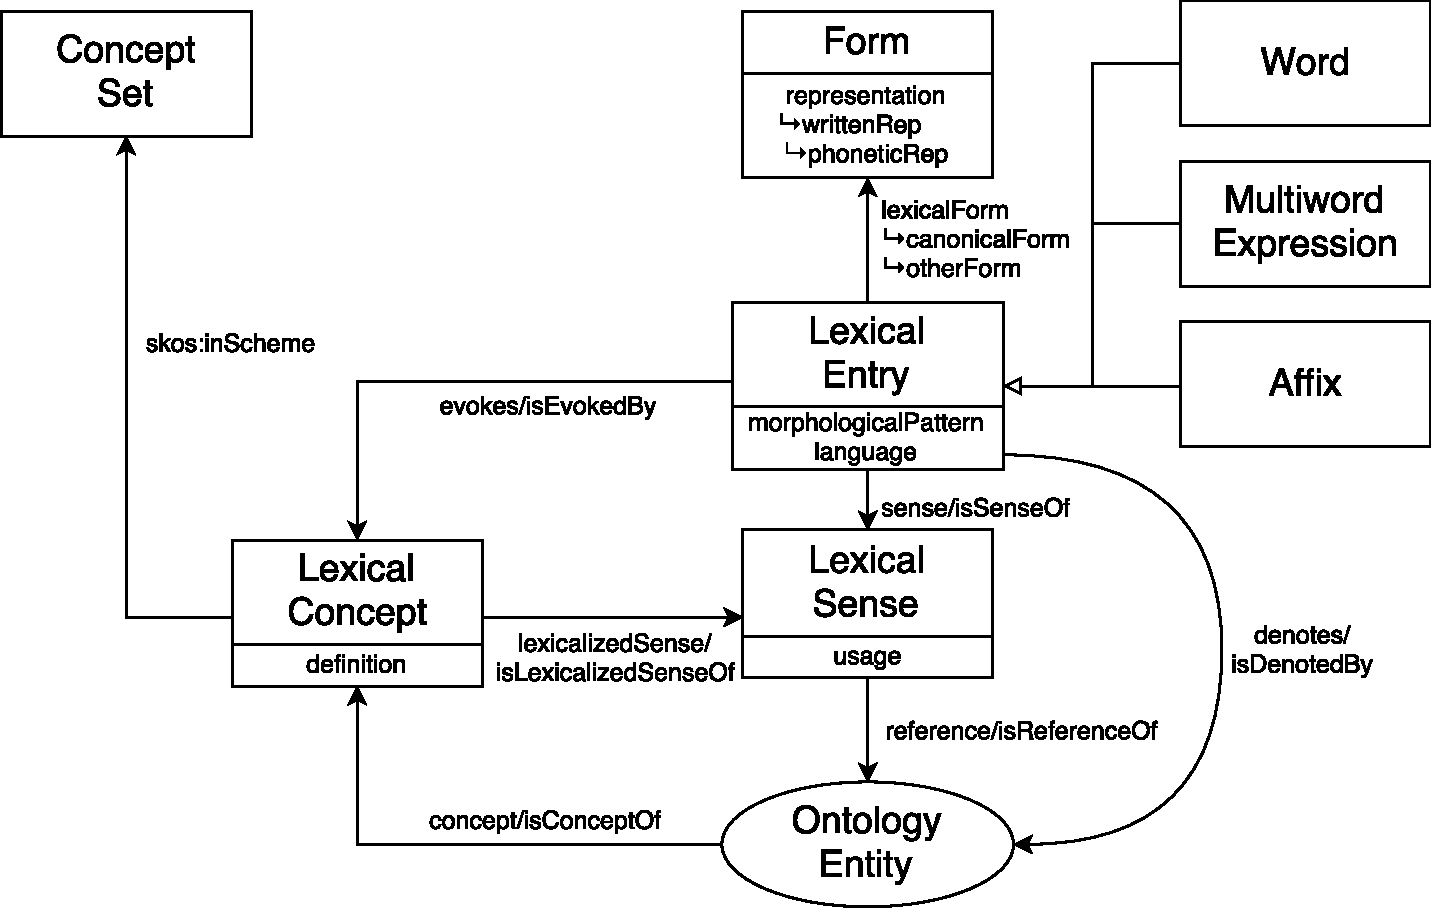
\includegraphics[width=0.8\textwidth]{LemonOntoLexCore.pdf}
    \end{center}
\caption{\label{fig:core}The Core Lemon OntoLex Model}
\end{figure}

Here we provide a brief summery of the Lemon OntoLex Model, for a more complete
description please see \cite{cimiano2016lexicon}.
The Lemon OntoLex model is based around the core module, as depicted in
Figure~\ref{fig:core}. The primary element of this is the \emph{lexical entry}
which represents a single word and thus collects together all morphological
expressions of that word, which correspond to \emph{forms} in the model, and all
possible concepts in the ontology it can refer to, which correspond to
\emph{lexical senses} in the model. It is important to note that the actual
meaning of a word is given by reference to an ontological concept and
\emph{lexical senses} represent only the mapping from a word to a concept. In
contrast to the previous \emph{lemon} model, a third semantic element called the
\emph{lexical concept} was introduced that allows for a meaning to be defined
independently of an ontology. For example, the verb `to die' may refer to
different ontological properties such as \texttt{deathDate} and \texttt{deathPlace} while
still referring to a single concept of \emph{Dying}. The model also supports
some other features including marking the canonical form (lemma), whether an
expression is a multiword expression and giving a \emph{usage} condition
describing when a particular word expresses a given concept (for example the
register), which is annotated on the lexical sense showing its role in giving a
mapping between concepts.


In addition to the core, there are four modules defined by the specification:

\begin{description}
    \item[Syntax and Semantics] The syntax and semantics module describes how
        particular lexical constructs, e.g., verb frames, can be mapped to
        constructs in the ontology. As a simple example, this concerns how a
        transitive verb frame such as `X knows Y' can be mapped to the subject
        and object arguments of a property such as \texttt{A foaf:knows B}. In this
        case there are only two options based on whether the grammatical subject
        (X) refers to property's subject (A) or object (B), however more complex
        multi-argument structures are also convered.
    \item[Decomposition] The decomposition module allows for multiword lexical
        entries to be decomposed into individual words, which are also
        represented as \emph{components}. Components are allowed to be marked
        with their own grammatical properties and are said to \emph{correspond
        to} either a lexical entry (i.e., for the word), an argument in a frame
        or another frame (to model phrasal arguments). 
    \item[Variation and Translation] The variation and translation model
        represents relationships between words at three levels: (purely)
        lexical, sense (lexico-semantic) and conceptual. These correspond
        to the levels of the model, with lexical relations being between lexical
        entries and such not considering the meaning of a word and only its
        syntactic properties. Similarly a conceptual relationship is between a
        lexical conceptual and does not consider the lexical form and hence
        language of a relation. Sense relations required knowledge of
        both the word form and the meaning and translation is thus considered a
        special case of a sense relation. The module also allows technical
        modelling of a relation either as a single triple or as a
        dereferenceable entity in itself, which allows for further annotation of
        metadata about the link.
    \item[Metadata (Lime)] The Linguistic Metadata (Lime) module adds modelling
        for grouping sets of lexical entries together into a lexicon and
        providing simple metadata such as the number of entries, senses, etc.
        Note that as linked data is intended to be published on the Web together
        the necessity to have all words grouped into a lexicon is not considered
        a core but still a useful feature.
\end{description}

\section{Use cases}

\subsection{Representing dictionaries with OntoLex}

\textbf{Julia?}

\subsection{The Collaborative Interlingual Index}

Princeton WordNet (PWN, \cite{fellbaum2010wordnet}) is the most widely used
lexicographic resource for natural language processing, but yet is only
available for English. There have been many versions of wordnets for other
langauges and these have been collected together in the Open Multilingual
WordNet~\citep{bond2013linking}, however they have primarily been created by the
\emph{extend approach}, where existing synsets from Princeton WordNet have been
translated and then new synsets are added for words which do not exist in
English. Unfortunately, this has led to a degree of fragmentation, where certain
concepts may be independently defined by different wordnets. In order to fix
this issue, it has been proposed that all wordnets contribute to a single index
of concepts~\citep{pease2008building}. This has recently been realized by the
Collaborative Interlingual Index (CILI, \cite{bond2016cili}), in which all
wordnets are converted to a common format and linking is made between the
synsets. In order to do this, it is assumed that each concept must have both an
English definition and a link to a synset already defined in the CILI. 

\begin{figure}
    \footnotesize
    \begin{verbatim}
{ 
  "@context": "http://globalwordnet.github.io/schemas/wn-json-context-1.0.json",
    "@graph": [{
      "@context": { "@language": "en" },
      "@id": "example-en",
      "@type": "ontolex:Lexicon", 
      "label": "Example wordnet (English)",
      "language": "en",
      "email": "john@mccr.ae",
      "rights": "https://creativecommons.org/publicdomain/zero/1.0/",
      "version": "1.0",
      "entry": [{
          "@id": "w1",
          "lemma": { "writtenForm": "grandfather" },
          "partOfSpeech": "noun",
          "sense": [{
              "@id": "example-en-10161911-n-1",
              "synset": "example-en-10161911-n"
          }]
      }],
      "synset": [{
          "@id": "example-en-10161911-n",
          "ili": "i90287",
          "partOfSpeech": "noun",
          "definition": [{
              "gloss": "the father of your father or mother"
          }],
          "relations": [{
              "relType": "hypernym",
              "target": "example-en-10162692-n"
          }]
      }]
  }]
}
    \end{verbatim}
    \caption{\label{fig:json-example}An example WordNet in the Global WordNet
    JSON-LD format}
\end{figure}



In order to, implement this it has been necessary to define a common format for
the definition of
wordnets\footnote{\url{https://globalwordnet.github.io/schemas}}. This format
allows for three forms: XML, JSON and RDF, all of which can be converted without
any loss of information. The XML format is based on the existing Lexical Markup
Framework~\citep{francopoulo2006lexical} and in particular on the WordNet-LMF
variant~\citep{soria2009wordnet}. Both the JSON and RDF formats are based on this
OntoLex model described in this paper, and the RDF version of this format is
considered a limited \emph{profile} of the OntoLex model, suited particularly
for the case of representing wordnets. The JSON version more precisely defines
its semantics by means of a JSON-LD context~\citep{sporny2014json}. An example
of this is given in Figure~\ref{fig:json-example}, in which the term
``grandfather'' is defined. In this example, a number of required standard
metadata properties are defined using widely-used vocabularies, namely Dublin
Core~\citep{rfc2413} and
Schema.org\footnote{\url{https://webmasters.googleblog.com/2011/06/introducing-schemaorg-search-engines.html}}.
Then the file contains two sections \texttt{entry} and \texttt{synset}, which
define the \emph{lexical entries} and \emph{lexical concepts} in this lexicon.
They both have a part-of-speech property, with specific values defined in a
custom WordNet
ontology\footnote{\url{http://globalwordnet.github.io/schemas/wn}}. The senses
of the model correspond to the \emph{lexical senses} of the OntoLex
model. For synset and sense relations the variation modules is used that enables
relationships between senses to be further described with metadata.

The use of linked data to represent the interlingual index has a number of
advantages, most specifically that each ILI identifier is associated with a
unique URL, where further information about the term can be found. For example,
for \texttt{i1234} information about this resource can be obtained at
\url{http://ili.globalwornet.org/ili/i1234}, including the definition of the
concept in English as well as links to the Princeton WordNet and other wordnets
who have contributed their links to the ILI. The URL thus allows for a stable
identifier that can be referred to unambiguously as opposed to the current
method of referring to offsets in release files.

\section{Extensions and Future Plans}

The OntoLex Community Group released its ``final report'' on the
10\textsuperscript{th} May 2016,
however the work of the group has not yet stopped and the group has an ambition
to develop more modules in response to critical analysis and novel uses case
(such as \cite{chavula2014lemon}). In particular, the group has recently aimed
to develop four new modules in order to further extend the applicability of the
model:

\begin{description}
    \item[Morphology] The first \emph{lemon} proposal contained a module for
        ``inflectional and agglutantive morphology'', which primarily defined
        morphological processes by means of regular expressions. This
        methodology was very simple to implement in any programming language
        that support Perl-like regular expressions, however does not very
        accurately represent the phonological process that occur in word
        morphology. As such, under this model certain regular cases like the
        plural of `leaf' to `leaves' would be modelled as distinct morphological
        paradigms even though it is generally considered part of the normal paradigm of
        pluralization in English. Thus the original model was not included in
        the Lemon OntoLex model and has been made available as
        a standalone ontology called LIAM (Lemon Inflectional Agglutinative
        Morphology)\footnote{\url{http://lemon-model.net/liam}}. There have
        since been a number of new proposals for morphology and in particular
        the group is discussing the adoption of the MMoOn Ontology of
        \citep{MMoOn_heb}. \textbf{TODO: More here}
    \item[Lexicography] \textbf{Jorge?}
    \item[Etymology and Diachronicity] Some authors~\citep{khan2014using,abromeit2016linking} have
        proposed using the OntoLex model to represent dictionaries of historical
        languages, and moreover most dictionaries contain some etymological
        information. As such, the ability of a dictionary to represent the
        change of lexical items over time is important. Thus, it has been
        recognized that the development of a module to capture meaning of words
        over time is a key use case of the model.
    \item[Lexico-syntactic categories] The OntoLex Model follows a principle of
        avoiding prescriptive modelling, for example allowing individual models
        to define their own categories. This is helpful as in the example
        of part-of-speech values in wordnets discussed above, where this
        approach allows the resource to define categories that may not be
        accepted by other lexicographers\footnote{In particular, Princeton
        WordNet defines `adjective satellite' as a distinct category to
        `adjective'}. However, the definition of standard categories greatly
        helps interoperability between resources and the LexInfo
        ontology~\citep{cimiano2011lexinfo} has been used by a number of authors
        for this
        purpose~\citep{buitelaar2013linguistic,villegas2015parole,serasset2015dbnary}. 
        This resource, originally derived from the
        ISOcat~\citep{kemps2008isocat} categories, is currently maintained as a
        single OWL file. As such, the group aims to re-evaluate this model and
        add establish a procedure for adding new categories to a single
        ontology. This will still only be a suggestion for data categories
        and we expect particular communities to define their own ontologies.
\end{description}

\section{Conclusion}

The OntoLex Model has been developed under an open process and as such
represents on the most significant open models for the representation of
electronic lexicographic resources. While the model as proposed has remained
close to the proposal of \cite{mccrae2012interchanging}, it has also
significantly innovated in order to allow new use cases. In particular, the
application of the model beyond the Semantic Web community has required new
modelling, in particular the introduction of \emph{lexical concepts} and
dereferenceable relations. These developments have seen the model adapted in a
wider community and as such have consequently lead to requests for new features.
The group remains committed to developing the model and new use cases in
morphology and diachronic lexicography will further show the flexibility of this
linked data based model.

\section*{Acknowledgement} 

We would like to thank all members of the OntoLex group for their contributions
and discussion of the model. This work was supported in part by the Science Foundation Ireland under Grant
Number SFI/12/RC/2289 (Insight). \textbf{CITEC?} \textbf{UPM?}

\section*{References}

%\nocite{*}
\printbibliography[
    type={book},
    notkeyword={dictionary},
    title={Books}
]
\printbibliography[
    type={incollection},
    title={Book Sections}
]
\printbibliography[
    type={inproceedings},
    title={Paper in conference proceedings}
]
\printbibliography[
    type={article},
    title={Journal Articles}
]
\printbibliography[
    type={misc},
    title={Technical Reports}
]
\printbibliography[
    type={book},
    keyword={dictionary},
    title={Dictionaries}
]


\medskip
\begin{minipage}[t]{\textwidth}
    \noindent This work is licensed under the Creative Commons Attribution
    ShareAlike 4.0 International License.
    \vspace{-2ex}
    \begin{center}%
        \url{http://creativecommons.org/licenses/by-sa/4.0/}\linebreak
        
\includegraphics[width=2.33cm]{cc.png}%
    \end{center}
\end{minipage}

\end{document}
% vim: noai nocin nosi inde=:
